\paragraph{Architectural decisions} As most in similar systems, Aquarium's architectural design is driven by two 
requirements: scaling and fault tolerance. As described in the requirements
section above, the concurrency and responsiveness requirements are steep;

Driven by our former experience with 3 tier systems, we designed the first
Aquarium prototype around a traditional relational database backend, with an
object relational mapping ({\sc orm}) based middle layer that run the business
processes (billing, message processing etc) and a fully-fledged {\sc rest}
frontend. While the simplicity of {\sc orm} systems provided a great start,
it quickly became obvious that such a design was too rigid for an open 
ended system. Complications arised from the fact that it was too difficult
to describe versioned tree-based structures, such as the configuration {\sc dsl} 
(see Section~\ref{sec:dsl}) and to make sure that resource events were
described in an abstract way that would include all future system expansions.
Moreover, the single query that places Aquarium in the system's critical 
path (number of remaining credits) must be answered within a few (less than
10) milliseconds for a large number of concurrent requests, which means that
it must be somehow cached and automatically updated when new chargable 
resources are invoked by the user.

For the reasons outlined above, we chose to base Aquarium on event sourcing. 
Event sourcing assumes that all changes to application
state are stored as a sequence of events, in an immutable log. With such a log
at hand, a system can easily rebuild the current state by replaying the events
in order. The event sourcing design pattern has some very interesting
properties, which made it particularity suitable for basing Aquarium's
architecture on it:

\begin{itemize}

    \item Multiple models can be used in order to process the events, 
        concurrently. This means that Aquarium can provide a limited
        data view to its {\sc rest api} and a more detailed one to a
        helpdesk frontend.

    \item It is possible to perform queries on past system states by stopping
        the event replay at a certain point of interest. This would prove very
        possible for a future debugging interface.

    \item In a carefully implemented event sourcing system, application crashes 
        are not destructive, as long as event replay is fast enough and no
        state is inserted to the application without being recorded to the event
        log first.

    \item After event log replay, new events only cause updates in the system's
        in-memory state, which can be done very fast.

\end{itemize}

\begin{figure}
    \begin{center}
    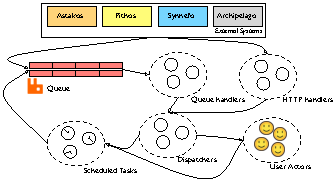
\includegraphics[scale=1.5]{arch.pdf}
    \end{center}
\caption{Functional components in Aquarium's architecture} 
\label{fig:arch}
\end{figure}

With event sourcing as the basis for Aquarium, we then proceeded to design the
system's runtime data model. What we wanted to model was the current state of
resource usage for each user, along with the user's wallet. One possibility we
wanted to explore on that front was copy on write updates; even for trivial
updates, the system would have to copy the affected data graphs to new
versions, instead of modifying the system in place. For that, we briefly
explored the use of software transactional memory, but found it restrictive for
our pursposes. What we chose instead was to contain each user's runtime state
in an actor. Using this design, shared state was eliminated; the use of the
actor model guarantee, that only one thread can execute within the context of
an actor renders the protection (with copy on write or other mechanism) of the
actor's state superflous. The actor model also fitted the event sourcing basis
very well, since each message in the log could pass through various processing
stages and reach the appropriate actor immutably.

\paragraph{Components} An overview of the Aquarium architecture is presented in
Figure~\ref{fig:arch}.  The system is modeled as a collection of logically and
functionally isolated components, which communicate by message passing. Withing
each component, a number of actors take care of concurrently processing
incoming messages through a load balancer component which is the gateway to
requests targeted to the component. Each component is also monitored by its own
supervisor; should an actor fail, the supervisor will automatically restart it.
The architecture allows certain application paths to fail individually while
the system is still responsive, while also enabling future distribution of
multiple components on clusters of machines.

The system receives input mainly from two sources: a queue for resource and
user events and a {\sc rest api} for billing state queries. The queue component
reads messages from a configurable number of queues and persists them in the
application's immutable log store. Both input components then forward incoming
messages to a network of dispatcher handlers which do not do any processing by
themselves, but know where the user actors lay. As described earlier, actual
processing of billing events is done within the user actors. Finally, a
separate network of actors take care of scheduling periodic tasks, such as
refiling of user credits; it does so by issuing events in the appropriate
queue.

\paragraph{Implementation}

Aquarium is being developed as a standalone service, based on the Akka library
for handling actor related functionality. Akka has all basic components for
implementing the architecture as described, which allowed us to focus on
implementing the business logic, leaving the details of actor registries,
dispatchers and message passing to Akka's runtime. Akka also provided
actor-based components for communicating with the message queue and, through a
third party component (Spray)\footnote{\url{http://github.com/spray}} for
handling {\sc rest} requests.  We chose the {\sc amqp} protocol and its
Rabbit{\sc mq} implementation for implementing the request queue, specifically
because recent versions include support for active/active cluster
configurations. The persistence layer is currently implemented by Mongo{\sc
db}, for its replication and sharding support.  However, this is not a hard
requirement, as Aquarium features an abstraction layer for all database queries
(currently 10 methods), which can then be implemented by any persistence
system, relational or not.
